\section{NCut谱划分}
\label{sec:graph-ncut}

RatioCut在割权相同时偏好顶点数较均衡的划分，但顶点数不反映每个顶点参与连接的多少。例如，把星图的多个叶子归为一组，这组顶点内部没有边，其全部度数都来自跨组连接。若希望比较每侧跨组连接占该侧总连接量的比例，可以把分母换成集合体积。体积包括内部边和跨割边的贡献，不能直接等同于内部边权或内部连接密度。

为此，Shi与Malik于2000年提出将RatioCut分母中的“节点个数$|A|,|B|$”替换为子图中所有节点的\emph{度数之和}（即第~\ref{sec:graph-conductance}小节定义的集合体积$\operatorname{vol}(A),\operatorname{vol}(B)$），从而得到了\term{归一化割}（normalized cut，简称\term{NCut}）\scite{shi2000normalized}。

以下先限制在正度顶点集$V_+$上，并假定$V_+$非空；无自环图中这保证$|V_+|\geq2$。若全图没有正权边，则不存在两侧均为正体积的合法NCut划分。

\subsection{NCut的谱松弛}
\label{sec:graph-ncut-relaxation}

\begin{definition}[NCut目标]
\label{def:graph-ncut}
设非空二分$(A,B)$（其中$B=V\setminus A$）两侧的体积分别为$\operatorname{vol}(A)=\sum_{i\in A}d_i>0$和$\operatorname{vol}(B)=\sum_{j\in B}d_j>0$（满足$\operatorname{vol}(A)+\operatorname{vol}(B)=\operatorname{vol}(V)$）。划分$(A,B)$的归一化割（NCut）目标定义为
\begin{equation}
\label{eq:graph-ncut}
\operatorname{NCut}(A,B)
=\frac{c(A,B)}{\operatorname{vol}(A)}+\frac{c(A,B)}{\operatorname{vol}(B)}
=c(A,B)\left(\frac{1}{\operatorname{vol}(A)}+\frac{1}{\operatorname{vol}(B)}\right).
\end{equation}
\end{definition}

由$\operatorname{vol}(A)=2w(E(A))+c(A,B)$可得，当$c(A,B)/\operatorname{vol}(A)$较小时，$A$的度数总和主要来自内部边；另一侧同理。因此，NCut较小表示两侧各自只有较小比例的连接权重通向外部，并不保证内部连通或内部边密度较高。全图体积固定时，体积平衡也是目标的一部分，但不能同时独立最大化两侧体积。

\begin{BookInlineFigure}
  \centering
  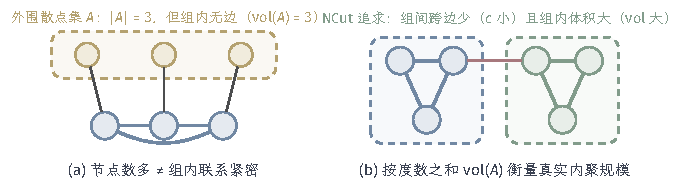
\includegraphics[width=114.935mm]{figures/03-graphs/05-matrices-and-spectra/tikz/ncut-volume-vs-count/figure.pdf}
  \caption{为什么NCut用度数总和（体积$\operatorname{vol}(A)$）替代节点个数$|A|$。(a) 将$3$个外围叶子归为集合$A$时，虽然节点数$|A|=3$已占半图，但$A$内部没有一条边，体积仅为$\operatorname{vol}(A)=3$。(b) 将两个内部紧密相连的三角形社区切开时，仅断开$1$条红边，而两侧体积各达$\operatorname{vol}=7$，两侧的跨割权与体积之比均为$1/7$。}
  \label{fig:graph-ncut-volume-vs-count}
\end{BookInlineFigure}

与第~\ref{sec:graph-ratiocut-relaxation}小节的RatioCut推导完全平行，只需把顶点个数$|A|,|B|$替换为集合体积$\operatorname{vol}(A),\operatorname{vol}(B)$，并把标准欧氏内积替换为以度矩阵$\bm D$加权的内积，即可分四步导出NCut的谱松弛。

\paragraph{1. 构造按体积加权的指示向量$\bm f$}

对任意满足$\operatorname{vol}(A)>0,\operatorname{vol}(B)>0$的二分$(A,B)$，利用两侧体积的比值构造两值指示向量$\bm f=(f_1,\ldots,f_n)^\top\in\mathbb R^n$：
\begin{equation}
\label{eq:ncut-indicator-vector}
  f_i = \begin{cases}
    \sqrt{\dfrac{\operatorname{vol}(B)}{\operatorname{vol}(A)}}, & i\in A,\\[10pt]
    -\sqrt{\dfrac{\operatorname{vol}(A)}{\operatorname{vol}(B)}}, & i\in B.
  \end{cases}
\end{equation}

\paragraph{2. 代入二次型分子$\bm f^\top\bm L\bm f$}

将$\bm f$代入组合拉普拉斯二次型$\bm f^\top\bm L\bm f=\sum_{\{i,j\}\in E}w_{i,j}(f_i-f_j)^2$。组内边两端取值相同、差为$0$；每条跨割边两端取值差的平方为
\[
\begin{aligned}
  \left(\sqrt{\frac{\operatorname{vol}(B)}{\operatorname{vol}(A)}} - \left(-\sqrt{\frac{\operatorname{vol}(A)}{\operatorname{vol}(B)}}\right)\right)^{\!2}
  &= \frac{\operatorname{vol}(B)}{\operatorname{vol}(A)} + \frac{\operatorname{vol}(A)}{\operatorname{vol}(B)} + 2 \\
  &= \operatorname{vol}(V)\left(\frac{1}{\operatorname{vol}(A)}+\frac{1}{\operatorname{vol}(B)}\right).
\end{aligned}
\]
对所有跨割边加权求和，得到二次型分子：
\begin{equation}
\label{eq:ncut-quadratic-numerator}
  \bm f^\top\bm L\bm f = \operatorname{vol}(V)\,c(A,B)\left(\frac{1}{\operatorname{vol}(A)}+\frac{1}{\operatorname{vol}(B)}\right)
  = \operatorname{vol}(V)\,\operatorname{NCut}(A,B).
\end{equation}

\paragraph{3. 验证度加权分母和度加权正交条件}

由于式~\eqref{eq:ncut-indicator-vector}使用的是体积比值，对应的正交条件和范数分母也自然带有顶点度数$d_i$的权重（即度对角矩阵$\bm D$）。第一，计算度加权坐标和$\bm f^\top\bm D\bm 1$：
\[
\begin{aligned}
  \bm f^\top\bm D\bm 1
  = \sum_{i=1}^n d_i f_i
  &= \left(\sum_{i\in A}d_i\right)\sqrt{\frac{\operatorname{vol}(B)}{\operatorname{vol}(A)}}
    - \left(\sum_{j\in B}d_j\right)\sqrt{\frac{\operatorname{vol}(A)}{\operatorname{vol}(B)}} \\
  &= \sqrt{\operatorname{vol}(A)\operatorname{vol}(B)} - \sqrt{\operatorname{vol}(A)\operatorname{vol}(B)}
  = 0.
\end{aligned}
\]
即向量$\bm f$恒满足度加权零和条件$\bm D\bm 1\perp\bm f$。

第二，计算度加权长度平方（分母$\bm f^\top\bm D\bm f$）：
\[
\begin{aligned}
  \bm f^\top\bm D\bm f
  = \sum_{i=1}^n d_i f_i^2
  &= \operatorname{vol}(A)\cdot\frac{\operatorname{vol}(B)}{\operatorname{vol}(A)}
    + \operatorname{vol}(B)\cdot\frac{\operatorname{vol}(A)}{\operatorname{vol}(B)} \\
  &= \operatorname{vol}(B) + \operatorname{vol}(A)
  = \operatorname{vol}(V).
\end{aligned}
\]
将分子式~\eqref{eq:ncut-quadratic-numerator}除以分母$\bm f^\top\bm D\bm f=\operatorname{vol}(V)$，常因子$\operatorname{vol}(V)$消去，得到广义Rayleigh商恒等式：
\begin{equation}
\label{eq:ncut-rayleigh-identity}
  \operatorname{NCut}(A,B) = \frac{\bm f^\top\bm L\bm f}{\bm f^\top\bm D\bm f}.
\end{equation}

\paragraph{4. 等价变换与连续松弛}

离散NCut问题要求$f_i$取式~\eqref{eq:ncut-indicator-vector}中由划分确定的两个值。放宽这一离散限制、允许$\bm f\in\mathbb R^n$取任意满足$\bm f^\top\bm D\bm 1=0$的非零实向量，并在正度顶点空间上作可逆坐标变换$\bm z=\bm D^{1/2}\bm f$（即$\bm f=\bm D^{-1/2}\bm z$），则正交约束$\bm f^\top\bm D\bm 1=0$化为$\bm z\perp\bm D^{1/2}\bm 1$，目标函数化为对称归一化拉普拉斯$\mathcal L=\bm D^{-1/2}\bm L\bm D^{-1/2}$的标准Rayleigh商：
\begin{equation}
\label{eq:ncut-spectral-relaxation}
  \min_{\substack{\bm f^\top\bm D\bm 1=0\\\bm f\neq\bm 0}}\frac{\bm f^\top\bm L\bm f}{\bm f^\top\bm D\bm f}
  = \min_{\substack{\bm z\perp\bm D^{1/2}\bm 1\\\bm z\neq\bm 0}}\frac{\bm z^\top\mathcal L\bm z}{\bm z^\top\bm z}
  = \mu_2(\mathcal L).
\end{equation}
由此可知：NCut连续松弛问题的最小值恰为对称归一化拉普拉斯的第二小特征值$\mu_2(\mathcal L)$；若达到$\mu_2(\mathcal L)$的特征向量为$\bm z_2$，则还原到原顶点空间的连续最优解为$\bm f^\star=\bm D^{-1/2}\bm z_2$，它直接满足广义特征方程$\bm L\bm f^\star=\mu_2\bm D\bm f^\star$（即随机游走归一化拉普拉斯特征方程$\bm L_{\mathrm{rw}}\bm f^\star=\mu_2\bm f^\star$）。

\begin{theorem}[NCut的度加权二次型表示与谱松弛下界]
\label{prop:graph-ncut-relaxation}
对任意两侧体积均为正的划分$(A,B)$，按式~\eqref{eq:ncut-indicator-vector}定义的指示向量$\bm f$（或其度加权单位化向量$\bm f_A=\bm f/\sqrt{\operatorname{vol}(V)}$）满足$\bm f^\top\bm D\bm 1=0$且$\operatorname{NCut}(A,B)=\frac{\bm f^\top\bm L\bm f}{\bm f^\top\bm D\bm f}$。因而，所有合法二分的离散最优值$\operatorname{OPT}_N=\min_{\operatorname{vol}(A),\operatorname{vol}(B)>0}\operatorname{NCut}(A,B)$以正度顶点集上对称归一化拉普拉斯$\mathcal L$的第二小特征值$\mu_2$为下界：
\[
  \mu_2(\mathcal L)
  = \min_{\substack{\bm f^\top\bm D\bm 1=0\\\bm f\neq\bm 0}}\frac{\bm f^\top\bm L\bm f}{\bm f^\top\bm D\bm f}
  = \min_{\substack{\bm z\perp\bm D^{1/2}\bm 1\\\lVert\bm z\rVert_2=1}}\bm z^\top\mathcal L\bm z
  \leq \operatorname{OPT}_N.
\]
\end{theorem}

注意$\mu_2$始终在正度顶点集$V_+=\{i\in V:d_i>0\}$上计算：度数为$0$的孤立顶点既不贡献割权也不贡献体积，可在正度顶点划分完毕后归入任意一侧。

\subsection{算法实现}
\label{sec:graph-ncut-sweep}

\paragraph{主要思路与算法步骤}

NCut谱划分的整体框架与RatioCut一致，核心差别在于将矩阵从组合拉普拉斯$\bm L$换成了对称归一化拉普拉斯$\mathcal L=\bm D^{-1/2}\bm L\bm D^{-1/2}$，并且在求得$\mathcal L$的特征向量$\bm z_2$后，必须左乘$\bm D^{-1/2}$作\emph{坐标逆缩放还原}，得到原顶点空间上的谱坐标$\bm f=\bm D^{-1/2}\bm z_2$后再执行排序或聚类。

具体执行流程分为以下四步：
\begin{enumerate}
\item \emph{构建归一化拉普拉斯矩阵}：在正度顶点集上计算对称归一化拉普拉斯矩阵$\mathcal L = \bm D^{-1/2}\bm L\bm D^{-1/2} = \bm I - \bm D^{-1/2}\bm W\bm D^{-1/2}$。
\item \emph{求解归一化特征向量}：计算$\mathcal L$的第二小特征值$\mu_2$对应的特征向量$\bm z_2\in\mathbb R^n$（若作$k$路谱聚类，则求$\mathcal L$前$k$个最小特征值对应的特征向量$\bm z_1,\bm z_2,\ldots,\bm z_k$）。
\item \emph{坐标逆缩放与构建特征矩阵}：在二分问题中，将特征向量$\bm z_2$的每个分量除以对应顶点度数的平方根$\sqrt{d_i}$，还原为原顶点指示空间上的谱坐标向量$\bm f=\bm D^{-1/2}\bm z_2$（即$f_i=(\bm z_2)_i/\sqrt{d_i}$）；在$k$路谱聚类（Ng--Jordan--Weiss算法）中，将$\bm D^{-1/2}[\bm z_1,\ldots,\bm z_k]$（或直接将$[\bm z_1,\ldots,\bm z_k]$）的每一行归一化为单位长度行向量，构建特征矩阵$\bm V\in\mathbb R^{n\times k}$。
\item \emph{离散化还原（还原为最终切分）}：在二分问题中，将全部顶点按还原后的坐标$f_i$从大到小排序，依次扫描$n-1$个前缀切口，计算各自的$\operatorname{NCut}(S,\bar S)$并取最小值对应的划分输出（在$k$路划分中则对特征矩阵$\bm V$的行向量运行$k$-means聚类）。
\end{enumerate}

\begin{algorithm}[NCut谱划分]
\label{alg:graph-ncut-sweep}
给定正度支撑非空且连通的有限无向非负加权图$\mathcal G=(V,E,w)$，输出两侧为正体积的二分$(A,B)$及其NCut值。
\begin{enumerate}
\item \textbf{构建归一化矩阵}：在正度支撑上构建对称归一化拉普拉斯矩阵$\mathcal L=\bm D^{-1/2}\bm L\bm D^{-1/2}$。
\item \textbf{求解特征向量并还原坐标}：求$\mathcal L$的第二小特征值$\mu_2$对应的特征向量$\bm z_2$，作逆缩放还原$\bm f=\bm D^{-1/2}\bm z_2$（即$f_i=(\bm z_2)_i/\sqrt{d_i}$）。
\item \textbf{按还原坐标排序}：按$f_i$从大到小排列顶点，分量值相同的并列顶点整组跨过阈值。
\item \textbf{离散化还原（增量阈值扫描）}：按排序顺序逐组将顶点并入前缀集合$S$，用算法~\ref{alg:graph-ratiocut-sweep}的方式增量更新割权$c(S,\bar S)$，同时累加集合体积$\operatorname{vol}(S)=\sum_{i\in S}d_i$。对所有两侧体积均为正的候选$S$，按式~\eqref{eq:graph-ncut}计算$\operatorname{NCut}(S,\bar S)$（同时可记录导通率$\phi(S)$），返回NCut最小的划分$(A,B)$，并把原图孤点归入任意一侧。
\end{enumerate}
\end{algorithm}

\paragraph{为什么必须用还原后的$f_i$排序？}

在第二步到第三步中，有一个极易忽略的关键细节：对称矩阵特征求解器算出的是$\bm z_2$，而我们在式~\eqref{eq:ncut-indicator-vector}中构造的两值分组向量是$\bm f=\bm D^{-1/2}\bm z_2$。由于不同顶点的度数$d_i$不同，除以$\sqrt{d_i}$可能会反转两个顶点的先后顺序。

图~\ref{fig:graph-ncut-coordinate-order}用一个简单例子展示了这种顺序反转：设圆点顶点的真实谱坐标为$f_1=2$、度数为$d_1=1$；方点顶点的真实谱坐标为$f_2=1$、度数为$d_2=9$。在乘以$\sqrt{d_i}$变换到$z_i=\sqrt{d_i}\,f_i$后，圆点坐标为$z_1=1\times 2=2$，而方点坐标变为$z_2=3\times 1=3$，大小顺序刚好颠倒。因此，阈值扫描必须严格使用逆缩放还原后的$f_i=(\bm z_2)_i/\sqrt{d_i}$排序（这与第~\ref{sec:graph-cheeger-sweep}小节Cheeger上界证明中的排序完全一致）。

\begin{BookInlineFigure}
  \centering
  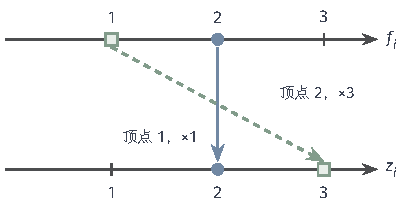
\includegraphics{figures/03-graphs/05-matrices-and-spectra/tikz/ncut-coordinate-order/figure.pdf}
  \caption{度数缩放可能改变顶点的排序先后。圆点对应度数$d_1=1$的顶点，方点对应度数$d_2=9$的顶点。按$z_i=\sqrt{d_i}\,f_i$转换到下轴时，方点坐标从$1$放大为$3$并反超圆点。阈值扫描必须使用上方的还原坐标$f_i$轴。}
  \label{fig:graph-ncut-coordinate-order}
\end{BookInlineFigure}

在单位权四点路径$1\!-\!2\!-\!3\!-\!4$上，各点度数为$(1,2,2,1)$，还原后的特征向量为$\bm f=(2,1,-1,-2)^\top$，按$f_i$从大到小排序仍为$1,2,3,4$。三个前缀候选切口的指标如下：切下$\{1\}$时割权为$1$、两侧体积为$1$和$5$，$\operatorname{NCut}=1\times(1+\frac15)=\frac65$；切断中间边得$\{1,2\}$时割权为$1$、两侧体积均为$3$，$\operatorname{NCut}=1\times(\frac13+\frac13)=\frac23$；切出$\{1,2,3\}$时$\operatorname{NCut}=\frac65$。算法返回中间割$\{1,2\}\mid\{3,4\}$，其NCut值$\frac23$夹在松弛下界$\mu_2=\frac12$之上。

\subsection{算法分析}
\label{sec:graph-ncut-guarantee}

记全图所有合法二分中的NCut真实最小值为$\operatorname{OPT}_N$，算法~\ref{alg:graph-ncut-sweep}扫描输出的划分为$S_N$。与RatioCut类似，松弛值$\mu_2$给出下界，扫描结果给出可行上界：
\begin{equation}
\label{eq:graph-ncut-bounds}
\mu_2(\mathcal L)\leq\operatorname{OPT}_N\leq\operatorname{NCut}(S_N,\bar S_N).
\end{equation}

NCut的松弛与阈值扫描使用的算子和坐标，与Cheeger不等式上界证明中的对象相同。由此可以得到不显式含最大度或最小度的目标值上界。下面分别核对目标函数、松弛方向和候选割之间的关系。

\paragraph{1. 目标函数同源：NCut与导通率$\phi(S)$仅差至多$2$倍}

对任意非空真子集$S\subsetneq V$，设两侧体积分别为$a=\operatorname{vol}(S)$和$b=\operatorname{vol}(\bar S)$，且不妨设$a\leq b$（即$a=\min\{\operatorname{vol}(S),\operatorname{vol}(\bar S)\}$）。对比定义~\ref{def:graph-conductance}与定义~\ref{def:graph-ncut}：
\[
\operatorname{NCut}(S,\bar S)
=\frac{c(S,\bar S)}{a}+\frac{c(S,\bar S)}{b}
=\frac{c(S,\bar S)}{a}\left(1+\frac{a}{b}\right)
=\phi(S)\left(1+\frac{a}{b}\right).
\]
由于$0<a\leq b$，比值$\frac{a}{b}$必定落在$(0,1]$内，故$1<\left(1+\frac{a}{b}\right)\leq 2$。因此，对图上的任何一个割，NCut与导通率$\phi(S)$都被锁定在常数$2$倍以内：
\begin{equation}
\label{eq:ncut-conductance-equivalence}
\phi(S)\leq\operatorname{NCut}(S,\bar S)\leq 2\phi(S).
\end{equation}

\paragraph{2. 谱松弛与扫描顺序完全一致}

对比式~\eqref{eq:graph-normalized-variational-cut}与式~\eqref{eq:ncut-spectral-relaxation}可以看到：Cheeger不等式所用的特征值$\mu_2(\mathcal L)$，与NCut连续谱松弛得到的下界$\mu_2(\mathcal L)$是\emph{同一个特征值}；而且第~\ref{sec:graph-cheeger-sweep}小节证明Cheeger上界时所扫描的特征向量$\bm f=\bm D^{-1/2}\bm z_2$，与算法~\ref{alg:graph-ncut-sweep}第三步排序所用的还原向量$\bm f=\bm D^{-1/2}\bm z_2$也是\emph{同一个向量}。换言之，NCut阈值扫描所考察的至多$|V_+|-1$个阈值前缀候选集，与Cheeger不等式上界证明所考察的前缀候选集完全相同。

\paragraph{3. 由Cheeger不等式直接导出NCut的性能保证}

由第~\ref{sec:graph-cheeger-sweep}小节的证明，同一批前缀候选中存在$S_\phi$使$\phi(S_\phi)\leq\sqrt{2\mu_2}$。算法在这些候选中最小化NCut，故$\operatorname{NCut}(S_N,\bar S_N)\leq\operatorname{NCut}(S_\phi,\bar S_\phi)$。再用$\operatorname{NCut}(S_\phi,\bar S_\phi)\leq2\phi(S_\phi)$和松弛下界$\mu_2\leq\operatorname{OPT}_N$，得到
\begin{equation}
\label{eq:graph-ncut-sweep-bound}
\begin{aligned}
\mu_2(\mathcal L)
&\leq \operatorname{OPT}_N
\leq \operatorname{NCut}(S_N,\bar S_N)
\leq \operatorname{NCut}(S_\phi,\bar S_\phi) \\
&\leq 2\phi(S_\phi)
\leq 2\sqrt{2\mu_2(\mathcal L)}
\leq 2\sqrt{2\operatorname{OPT}_N}.
\end{aligned}
\end{equation}

式~\eqref{eq:graph-ncut-sweep-bound}给出平方根形式的目标值保证。若$\operatorname{OPT}_N>0$，相除得到的近似因子为$2\sqrt{2/\operatorname{OPT}_N}$，并非常数；因此不能由此推断NCut在所有任务上优于RatioCut。得到准确谱向量后，排序与增量扫描共需$O(n\log n+m)$时间，特征向量求解的成本须另计。对于近似特征向量，还需根据其Rayleigh商和正交误差重新核对保证。

\begin{BookInlineFigure}
  \centering
  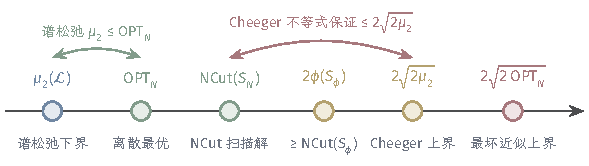
\includegraphics[width=99.713mm]{figures/03-graphs/05-matrices-and-spectra/tikz/ncut-sweep-and-cheeger-chain/figure.pdf}
  \caption{NCut谱划分与Cheeger不等式结合形成的双向近似保证链。左侧由连续谱松弛给出下界$\mu_2(\mathcal L)\leq\operatorname{OPT}_N$，右侧由Cheeger阈值扫描上界保证扫描输出解$S_N$满足$\operatorname{NCut}(S_N)\leq 2\sqrt{2\mu_2}\leq 2\sqrt{2\operatorname{OPT}_N}$。}
  \label{fig:graph-ncut-sweep-guarantee}
\end{BookInlineFigure}
